%% ============================================================
%% 片段：s05a-framework   对应原文 PDF 第 110--116 页
%% 本文件由 gw/convert.py 从 arXiv 源码（hep-th/0612073v2）自动生成：
%%   * 公式/编号/引用/图 已经锁定为原文内容，请勿改动任何数学内容与编号；
%%   * 只需把英文正文译为中文，并在每节开头加“本节重点”、关键处加译注。
%% ============================================================


\section{线算符与分歧}

%% ==== 原文 §5：PDF 第 110 页（印刷第 109 页）====
\label{sec:5}

\begin{keytakeaways}
  \begin{itemize}[leftmargin=1.4em,itemsep=2pt,topsep=2pt]
    \item \textbf{物理图像}：在四维流形 $M=\R\times W$（$W=I\times C$）上取时间无关的线算符与面算符，四维问题便化为三维流形 $W$ 上的静态图像：膜给出 $W$ 边界上的边界条件，线算符 $L_i=\R\times y_i$ 作用于膜，而面算符的支撑 $D=\R\times S$ 终止于边界，故属于膜的定义的一部分。
    \item \textbf{数学工具}：拓扑不变性使线算符可以自由移动，因而一般点处给出交换代数 ${\mathcal S}_{q}$；支撑在曲面上的线算符具有自然次序、无法彼此穿过，在分歧点处一般给出非交换代数 $\hat {\mathcal S}_p$，后者与 ${\mathcal S}_{q}$ 对易，且 ${\mathcal S}_{q}$ 沿 $q\to p$ 的（依赖于方向的）极限落入其中心。
    \item \textbf{关键结论}：$\Psi=\infty$ 处是复结构 $J$ 下的 $B$-模型（威尔逊算符保持 $(B,B,B)$ 型超对称），$\Psi=0$ 处是辛结构 $\omega_K$ 的 $A$-模型（'t Hooft 算符保持 $(B,A,A)$ 型超对称）；单值性只保持一个拓扑超对称，因而不是看到全部超对称的合适框架。在面算符的支撑上，$^L\neg G$ 约化为极大环面 $^L\neg \TT$，其表示环（即余权格）作用在膜上。
    \item \textbf{边界与展望}：在 $B$-模型中，半经典规范场论方法只能看到与平移 $\eta$ 对应的阿贝尔单值性，无法看到 $\Psi=\infty$ 处更大的非交换对称性；在 $A$-模型中 $\alpha$ 与 $\eta$ 的角色互换，因而更有希望，这是下一步的目标。
  \end{itemize}
\end{keytakeaways}

在第~\ref{sec:4.5}~节中，我们描述了分歧点处威尔逊算符与 't Hooft 算符的类似物。这一描述也许显得有些抽象，而答案——特别是在幂幺单值性（unipotent monodromy）的情形——却出人意料地复杂。相比之下，作用在 $C$ 上一般点处的威尔逊算符与 't Hooft 算符，通常是用颇为不同的规范场论方法定义的。

用完全不同的方法来描述这两种情形并不能令人满意，因此本节试图在分歧情形下给出一个规范场论的定义。这还有另一个好处：它将帮助我们理解这些算符的完全超对称（\mbox{supersymmetry}）。

紧化到二维后，在 $\Psi=\infty$ 处出现的拓扑场论是以复结构 $J$ 下的 $\MH$ 为靶空间的 $B$-模型（$B$-model）。第~\ref{sec:4.5}~节所考虑的单值性保持这一超对称。然而，非分歧点处相应的威尔逊算符保持更大的超对称：它们具有 $(B,B,B)$ 型的超对称，也就是说，它们保持 $B$-模型在构成 $\MH$ 的超 Kähler 结构的任一复结构下的超对称。

类似地，在 $\Psi=0$ 处，相应的拓扑场论是辛结构为 $\omega_K$ 的 $\MH$ 的 $A$-模型（$A$-model）。第~\ref{sec:4.5}~节所研究的单值性保持相应的超对称。然而，相应的 't Hooft 算符实际上保持 $(B,A,A)$ 型超对称，也就是说，它们保持类型 $I$ 的 $B$-模型以及类型 $J$ 或 $K$ 的 $A$-模型的超对称。

我们将力图用规范场论来证明：作用在分歧点处的相应算符确实与一般点处的威尔逊算符和 't Hooft 算符具有相同的超对称。对 $A$-模型我们能够实现这一点，对 $B$-模型则只能部分实现。

\begin{yizhu}[含糊点拨]
参数 $\Psi$ 标记所选取的拓扑扭曲：$\Psi\to\infty$ 与 $\Psi=0$ 分别给出复结构 $J$ 下的 $B$-模型和辛结构 $\omega_K$ 的 $A$-模型（在 \cite{ref8} 的记号中，相应的扭转参数为 $t$；$t=1$、四维 $\theta$ 角为零时得到 $\Psi=0$，见第~\ref{sec:5.3}~节）。原文说单值性“保持相应的超对称”，意思是它只保持其中一个拓扑超荷；而威尔逊算符与 't Hooft 算符保持得更多：前者保持三种复结构下 $B$-模型的超对称，即 $(B,B,B)$ 型；后者保持类型 $I$ 的 $B$-模型与类型 $J$、$K$ 的 $A$-模型的超对称，即 $(B,A,A)$ 型。单值性之所以不足以刻画这些算符，正在于此，这也是本节改用规范场论重新定义线算符的动机。
\end{yizhu}

\subsection{一般框架}
%% ==== 原文 §5.1：PDF 第 111 页（印刷第 110 页）====
\label{sec:5.1}

为简单起见，我们在四维流形 $M=\Sigma\times C$ 上工作。照例，$C$ 是研究几何朗兰兹纲领所在的黎曼面。取 $\Sigma=\R\times I$，其中 $\R$ 参数化“时间”，$I$ 是一闭区间。于是也可写 $M=\R\times W$，其中 $W=I\times C$ 是一个三维流形。膜被选取用来在 $W$ 的边界上定义边界条件。


% [FIGURE 2] 原文 PDF 第 111 页；caption 见下，需翻译
\begin{figure}[htbp]
  \centering
  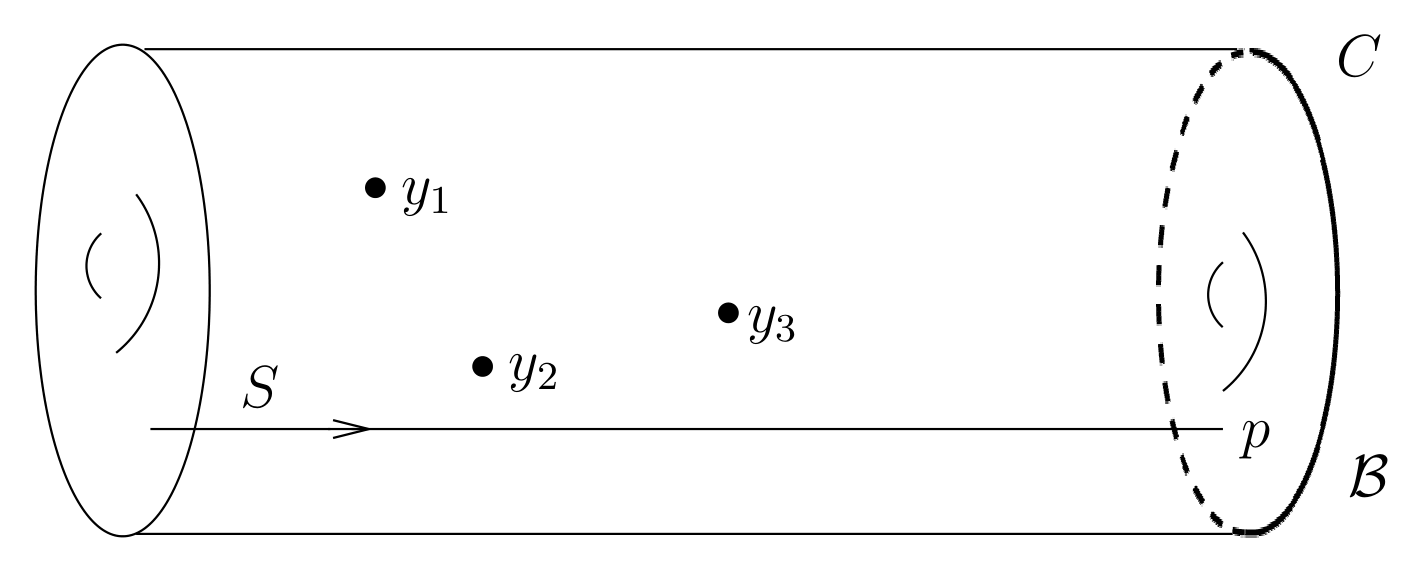
\includegraphics[width=0.62\linewidth]{figures/figure-2.png}
  \caption{时间无关情形的零时刻切片。面算符的支撑 $D$ 与零时刻切片的交为直线 $S$；若干线算符的支撑 $L_i$ 与零时刻切片交于点 $y_i$（$i=1,2,3$）。（原文 Fig.~2，PDF 第 111 页）}
  \label{fig:2}
\end{figure}


为简单起见，我们假定线算符（line operator）与面算符的支撑不依赖于时间。于是，只要说明 $W$ 中发生的情况，就能描述线算符与面算符的任何组态。时间无关的面算符支撑在二维流形 $D=\R\times S$ 上，其中 $S$ 是 $W$ 中的一条曲线。用于几何朗兰兹的分歧情形时，取 $S=I\times p$，其中 $p$ 是 $C$ 中的一点。我们还纳入支撑为 $L_i=\R\times y_i$ 的线算符，其中 $y_i\in W$ 是若干点。这些线算符将简记为 $L_i$。该组态如图~\ref{fig:2} 所示。

\begin{yizhu}[物理图像补充]
时间无关（time-independent）的假设并不失一般性：在拓扑场论中时间方向没有动力学，任意算符组态都可以沿时间方向推挤；若某个线算符或面算符的支撑在时间方向上只有有限延展，它就给出作用在膜上的算符（见上文脚注）。取 $\Sigma=\R\times I$ 后，$W=I\times C$ 是一个圆柱（图~\ref{fig:2}）；$S=I\times p$ 是沿圆柱的一条母线，其两端落在 $W$ 的两个边界上，因此面算符的支撑 $D=\R\times S$ 终止于边界，必须并入“膜”的定义，而不是作为作用在膜上的算符。这正是原文强调面算符与线算符地位不同的原因：线算符的支撑 $L_i=\R\times y_i$ 可以把端点推到边界，从而成为作用在膜上的算符，而面算符的支撑本身就终止于边界。
\end{yizhu}

线算符可以理解为作用在膜上的算符，详见 \cite{ref8} 第 6.4 节。例如，利用拓扑不变性，我们可以移动点 $y_i$，使其趋近图~\ref{fig:2} 中标记为膜 ${\mathcal B}$ 的右边界。当 $y_i$ 趋近边界时，相应的线算符 $L_i$ 作用在 ${\mathcal B}$ 上，给出一个新膜 ${\mathcal B}_i$，我们把它符号地记为 $L_i\cdot {\mathcal B}$。相反，由于 $S=I\times p$ 终止于 $W$ 的边界，支撑在 $D=\R\times S$ 上的面算符必须作为“膜”这一概念的定义的一部分；在这种情形下，它并不真正给出一个作用在膜上的算符。\footnote{若某线算符或面算符的支撑在时间方向上只有有限延展，则它会给出一个作用在膜上的算符。}

拓扑不变性意味着存在一个自然的平坦联络，使得支撑在点 $y_i\in W$ 处的线算符自然等价于支撑在邻近点 $y_i'$ 处的线算符。由此可知线算符彼此对易，因为三维流形中一个小开集内互异点位的组态空间是连通且单连通的。连通性意味着我们可以让两个线算符彼此穿过而不会遇到奇点；单连通性则意味着（在同伦意义下）如何这样做没有歧义。

\bigskip\noindent{\it 支撑在曲面上的线算符}


% [FIGURE 3] 原文 PDF 第 112 页；caption 见下，需翻译
\begin{figure}[htbp]
  \centering
  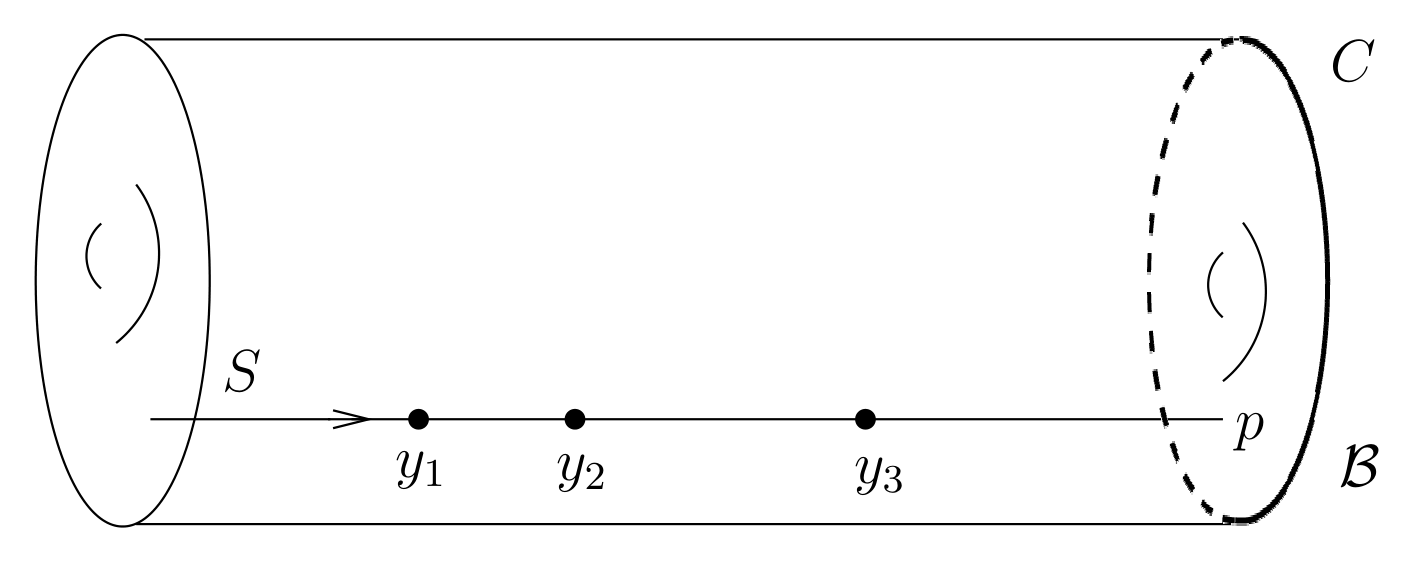
\includegraphics[width=0.62\linewidth]{figures/figure-3.png}
  \caption{支撑在曲面 $D$ 上的线算符 $L_i$。图中画出的是时间无关情形的零时刻切片；在零时刻，$D$ 由所示的直线 $S$ 表示，线算符则由 $S$ 上的点 $y_i$ 表示。（原文 Fig.~3，PDF 第 112 页）}
  \label{fig:3}
\end{figure}


然而现在考虑某些点 $y_i$ 实际落在曲线 $S$ 上的情形。在刚才的情形中，若取 $y_i=u_i\times p$，其中 $u_i\in I$、$p$ 是 $C$ 中的分歧点，就会出现这种情形（图~\ref{fig:3}）。此时，直线 $L_i=\R\times y_i$ 当然包含在曲面 $D=\R\times S$ 内，于是我们得到的是一个支撑在曲面上的线算符。当然，在给定面算符的支撑上允许何种线算符，是我们必须处理的一个问题。

支撑在曲面上的线算符与四维空间中的一般线算符颇为不同，因为只要定向适当，它们就具有自然的次序。图~\ref{fig:3} 画出了这一点，其中的次序为 $y_1<y_2<y_3$。支撑为 $\R\times y_i$ 的线算符给出一个作用在膜上的算符，因为我们可以把点 $y_i$ 向右移动，此时相应的线算符便作用在膜 ${\mathcal B}$ 上。然而一般来说，不应期望支撑在膜上的线算符彼此对易，因为它们有确定的次序，而且无法在不相遇奇点的情况下彼此穿过。

于是，在一般点 $q\in C$ 处，我们得到一个由作用在膜上的威尔逊算符或 't Hooft 算符构成的交换代数 ${\mathcal S}_{q}$。但在分歧点 $p$ 处，一般得到的是一个非交换代数 $\hat {\mathcal S}_p$。

尽管 $\hat {\mathcal S}_p$ 一般是非交换的，但它与支撑在一般点 $q\in C$ 处的威尔逊算符或 't Hooft 算符构成的代数 ${\mathcal S}_{q}$ 对易。道理很简单：只要 $q$ 不是分歧点，作用在 $q$ 处的线算符就可以自由地向左或向右移动，而不会遇到奇点。

\begin{yizhu}[易错点]
线算符与面算符的支撑是几何上不同的对象：一般线算符的支撑是 $L_i=\R\times y_i$（四维中的一条线，在零时刻切片上是点 $y_i$），面算符的支撑是 $D=\R\times S$（四维中的一个曲面，在切片上是曲线 $S$）。当 $y_i\in S$ 时 $L_i\subset D$，即线算符位于面算符的支撑之内；这类“支撑在曲面上的线算符”沿 $S$ 有自然次序（图~\ref{fig:3}，$y_1<y_2<y_3$），不能互相穿过，因此一般不对易。相反，$C$ 上一般点处的线算符可以自由移动，故交换。两种情形不可混为一谈：$\hat {\mathcal S}_p$ 的非交换性来自面算符支撑上的次序结构，而不是来自四维整体的拓扑。
\end{yizhu}

当然，非交换代数可能包含很大的中心。令 $q$ 趋近 $p$ 取极限，就可以把 ${\mathcal S}_{q}$ 映入 $\hat {\mathcal S}_p$ 的中心。在拓扑场论中，这一极限必定存在，因为 $q$ 与 $p$ 之间的距离本来就没有意义。不过，一般而言，当 $q$ 绕 $p$ 转过一周时会出现单值性；一旦如此，${\mathcal S}_{q}$ 中元素当 $q\to p$ 时的极限就依赖于逼近的方向。对 $B$-模型这一点是显然的（我们在第~\ref{sec:5.2}~节会提到），对 $A$-模型则已在 \cite{ref75} 中作了分析（所用的语言与本文颇为不同）。

因此，通常的威尔逊算符或 't Hooft 算符代数可以映入作用在分歧点处的非交换代数的中心，但并不完全以典范的方式。

\bigskip\noindent{\it 与单值性的关系}

下面讨论这一表述与第~\ref{sec:4.5}~节中用单值性所作描述之间的关系。在那种做法中，人们考虑的是只保持一个拓扑超对称的膜上操作——即复结构 $J$ 下 $B$-模型的对称性，或辛结构为 $\omega_K$ 的 $A$-模型的对称性。为简单起见，我们只以 $B$-模型来表述下面的论证。对 $A$-模型，只需把 $\alpha$ 与 $\eta$ 互换，情况完全相同。

在复结构 $J$ 下的 $B$-模型中，拉格朗日量对 Kähler 参数 $(\beta,\eta)$ 的依赖完全呈 $\int_M d^4x\sqrt g \{Q,V\}$ 的形式，其中 $Q$ 是相应的拓扑超荷，$V$ 选取适当。对控制复结构的参数 $(\alpha,\gamma)$ 的依赖则无法写成这种形式。

适当选取 $V$ 后，我们可以让 $(\beta,\eta)$ 这一对量成为沿面算符的支撑 $D$ 非常数的函数。就本文的目的而言，我们取这些函数不依赖于时间，但沿图~\ref{fig:3} 的曲线 $S$ 从左向右移动时发生变化。我们必须避开使量子理论变得奇异的那些 $(\beta,\eta)$ 取值。让 $(\beta,\eta)$ 沿 $S$ 变化并避开奇点轨迹，恰好重现第~\ref{sec:4.5}~节所描述的单值性。

现在可以看出单值性与线算符之间的关系。描述一个单值性时，可以令 $(\beta,\eta)$ 在某个小线段 $I_0\in S$ 之外为常数。在拓扑场论中，线段 $I_0$ 的长度无关紧要。若把该线段看作实质上是一个点，那么单值性不过是描述线算符的一种特殊方式。

然而，如果我们想看到 $\Psi=\infty$ 处 $B$-模型的全部拓扑超对称，用单值性来描述线算符就有缺陷。我们记得，这一对称性属于 $(B,B,B)$ 型。为了保持复结构 $J$ 下的 $B$ 型超对称，必须保持 $\alpha$ 与 $\gamma$ 固定（如上所做），因为该复结构依赖于这些参数。同样，为了保持复结构 $I$ 下的 $B$ 型超对称，必须保持 $\beta$ 固定，因为复结构 $I$ 依赖于 $\beta$。所以总的来说，要保持 $(B,B,B)$ 型的全部拓扑超对称，我们只能变化 $\eta$；而即便如此，最多也只能看到对应于把 $\eta$ 平移一个格矢量的阿贝尔单值性。

最有趣的非阿贝尔奇点预期出现在 $\alpha=\beta=\gamma=0$ 时。此时为避免奇点，$\eta$ 必须是正则的；于是 $\eta$ 被限制在一个仿射外尔房（affine Weyl chamber）的内部。在这一限制下，我们根本观察不到任何单值性。

当然，在 $\Psi=0$ 的 $A$-模型中，若想看到 $(B,A,A)$ 型的全部拓扑超对称，也有类似的问题。要保留问题的全部对称性，单值性就不是一个合适的框架。本节余下部分的目标是：看看改为从线算符而非单值性出发——也就是定义与非分歧情形中威尔逊算符和 't Hooft 算符类似的离散操作——能做得比单值性好多少。

\subsection{\texorpdfstring{$B$-模型}{B-模型}}

%% ==== 原文 §5.2：PDF 第 115 页（印刷第 114 页）====
\label{sec:5.2}

容易讨论的是 $B$-模型，但也正是在这一情形中我们无法得到完全令人满意的答案。

在非分歧情形，规范群为 $^L\neg G$ 时，作用在膜上的重要算符是 $^L\neg G$ 的表示 $^L\neg R$ 中的威尔逊算符。它们由复值联络 $\CA=A+i\phi$ 的平行移动（parallel transport）来定义。若 $L$ 是四维流形 $M$ 中的闭圈，则威尔逊算符定义为
% 式 (5.1)
\setcounter{equation}{0}
\begin{equation}\label{eq:5.1}
  W({}^L\neg
R;L)=\Tr\,P\exp\left(-\int_L\CA\right),
\end{equation}
 其中 $P\exp\left(-\int_L\CA\right)$ 是联络 $\CA$ 沿直线 $L$ 的和乐，迹在表示 $^L\neg R$ 中取。若 $L$ 改为一条开线（连接 $M$ 的边界或端点），则把 $W({}^L\neg R;L)$ 定义为此和乐，并将它视为在表示 $^L\neg R$ 的初态与末态之间作用的算符。

对非分歧情形的几何朗兰兹纲领，取 $M=\R\times I\times C$，其中 $\R$ 参数化“时间”，$I$ 是一个区间，$C$ 是黎曼面。要得到能作用在膜上的威尔逊算符，取 $L=\R\times u\times q$，其中 $u\in I$ 与 $q\in C$ 是选定的点。

若 $L$ 包含在面算符的支撑 $D$ 内（如图~\ref{fig:3}），我们可以作几乎相同的构造。但有一个重要差别：在面算符的支撑上，群 $^L\neg G$ 被约化为其极大环面 $^L\neg \TT$。因此，若 $L$ 包含在 $D$ 内，我们可以定义与 $^L\neg \TT$ 的表示的选择相应的威尔逊算符。这比选择 $^L\neg G$ 的表示更为一般，因为 $^L\neg G$ 的表示可以分解为 $^L\neg \TT$ 的表示的直和，但反过来一般不行。

因此一般说来，在分歧点处，$^L\neg \TT$ 的表示环（representation ring）作用在 $\Psi=\infty$ 处模型的膜上，从而推广了一般点处由 $^LG$ 的表示给出的作用。其发生方式很简单：与 $^LG$ 的表示相联系的、位于一般点 $q$ 的威尔逊算符，在 $q$ 趋近 $p$ 的极限下分裂为与 $^L\neg \TT$ 的表示相联系的威尔逊算符之和。

由于 $B$-模型的分歧平坦丛绕面算符的支撑具有单值性，这一情形中 $q\to p$ 的极限有微妙之处：极限依赖于人们让 $q$ 逼近 $p$ 所走的路径。

\bigskip\noindent{\it 解释}

$^L\neg \TT$ 的表示环就是余权格（coweight lattice）$\Lambda_\cowt$。其中包含一个由不改变离散电通量 ${\bf e}_0$ 的威尔逊算符组成的子格 $\Lambda_\cort$（余根格，coroot lattice）。

\begin{yizhu}[含糊点拨]
$^L\neg \TT$ 的表示环之所以等于余权格 $\Lambda_\cowt$，是因为 $\TT$ 与 $^L\neg \TT$ 互为对偶环面：$\TT$ 的余特征格正是 $^L\neg \TT$ 的特征格，而环面的不可约表示由特征（权）标号；等价地说，$^L\neg \TT$ 的表示环是以 $\Lambda_\cowt$ 为基的格代数。子格 $\Lambda_\cort$ 则对应不改变离散电通量 ${\bf e}_0$ 的那些威尔逊算符。原文没有展开的是：这一“表示环作用”与第~\ref{sec:4.5}~节由单值性给出的“格 $\Lambda_\cort$ 或 $\Lambda_\cowt$ 的作用”是同一件事的两种描述，其等价性依赖下面式~\eqref{eq:5.2} 的二维阿贝尔结果。
\end{yizhu}

我们在第~\ref{sec:4.5}~节中也遇到过格 $\Lambda_\cort$ 或 $\Lambda_\cowt$ 在膜上的作用。不过那里的解释稍有不同：在那种做法中，格的作用是平移 $\eta$，也就是把定义在杂质曲面（impurity surface）上的 $\theta$ 角平移 $2\pi$。

不过，一个经典结果 \cite{ref76} 表明：二维阿贝尔规范场论中的威尔逊算符会使 $\theta$ 角平移 $2\pi$ 的整数倍。下面回顾它是怎么来的。考虑二维流形 $D$ 上规范群为 $H=U(1)$ 的规范场论。取 $L$ 为 $D$ 上一条适当类型的一维流形。最简单的情形是 $L$ 为区域 $R\subset D$ 的边界，且是一条闭一维流形。设 $A$ 是 $D$ 上曲率为 $F$ 的阿贝尔规范场\footnote{我们把 $A$ 视为主 $U(1)$ 丛上的联络，局部地用实一维形式表示。}。则 $A$ 绕 $L$ 的和乐满足恒等式

% 式 (5.2)
\setcounter{equation}{1}
\begin{equation}\label{eq:5.2}
  \exp\left(i\oint_LA\right)=\exp\left(i\int_RF\right).
\end{equation}

这说明，在穿过支撑着电荷为 1 的威尔逊算符的那条线时，$\theta$ 角跳跃 $2\pi$。若分析得更仔细，即使一维流形 $L$ 不闭合，也能得到同样的结论。

\begin{yizhu}[易错点]
式~\eqref{eq:5.1} 与式~\eqref{eq:5.2} 的符号约定不同：式~\eqref{eq:5.1} 中 $\CA=A+i\phi$ 是复值联络，威尔逊线按本文约定取 $P\exp(-\int_L\CA)$（与 $D=d+A$、和乐 $P\exp(-\int A)$ 一致）；而式~\eqref{eq:5.2} 讨论的是按数学约定写成的 $U(1)$ 实一维形式 $A$，故用 $\exp(i\oint_LA)$。两者相差因子 $i$ 与符号，比较前必须统一约定。式~\eqref{eq:5.2} 的物理含义是：穿过电荷为 1 的威尔逊算符所在的线时 $\theta$ 角跳跃 $2\pi$；这也解释了为什么面算符支撑上“格的作用”既可看成表示环的作用，也可看成 $\eta$ 的平移（后者正是 $\theta$ 角的 $2\pi$ 平移）。
\end{yizhu}

\bigskip\noindent{\it 讨论}

因此，对于正则半单型单值性的情形，我们用规范场论找到的格在膜上的作用，就是我们预期能看到的全部。然而，按第~\ref{sec:4.5}~节的分析，当对 $(\alpha,\gamma)$ 非正则时，应当有一个更大的非交换群作用在膜上。遗憾的是，正如我们下面要说明的，在 $\Psi=\infty$ 处似乎很难用半经典规范场论方法看到这一更大的对称性。因此，用这些方法我们实际上无法比用单值性做得更好。

我们想看到的单值性来自 $\beta$ 与 $\eta$ 的变化；若把 $\beta$ 约束住，使三元组 $(\alpha,\beta,\gamma)$ 恒为正则，这些单值性就不存在。所以这些单值性的存在取决于该三元组变为非正则时发生的情况。此时，用第~\ref{sec:3.6}~节的话说，经典模空间 $\MH$ 会出现局部奇点。

这些单值性仍然有意义，因为只要 $\eta$ 是一般的，量子理论就保持光滑。然而，在线算符的半经典规范场论构造中，很难利用量子理论的这一事实。任何这类构造都从经典构造出发，然后在量子层面实现。定义依赖于理论量子性质的算符，用规范场论方法很难看到。

在 $A$-模型中情况不同，因为 $\alpha$ 与 $\eta$ 的角色互换了。相应的单值性通过在固定 $\gamma$ 与 $\eta$ 的同时变化 $\alpha$ 与 $\beta$ 而得到。即使 $\gamma=\eta=0$，只要 $(\alpha,\beta)$ 处于正则区域，就能看到全部单值性；而这意味着 $\MH$ 的经典几何是光滑的。

这提示我们，在 $A$-模型中，用规范场论方法描述作用在膜上的全部算符以及它们所保持的全部超对称，可能会更成功。这将是我们下一个目标。
